\documentclass[10pt,a4paper]{book}
\usepackage[utf8]{inputenc}
\usepackage{amsmath}
\usepackage{amsfonts}
\usepackage{amssymb}
\usepackage{pifont}
\usepackage{graphicx}
\usepackage[left=2cm,right=2cm,top=2cm,bottom=1.5cm]{geometry}
\usepackage{xcolor}
\usepackage[square,sectionbib]{natbib}
\usepackage{hyperref}
\usepackage{tabu}
\usepackage{threeparttable}
\usepackage{graphicx}

\definecolor{light-gray}{gray}{0.95}
%\newcommand{\code}[1]{\colorbox{light-gray}{\texttt{#1}}}
\newcommand{\option}[1]{{\texttt{'#1'}}}
\newcommand\tab[1][.6cm]{\hspace*{#1}}
\newcommand{\cmark}{\ding{51}}%
\newcommand{\xmark}{\ding{55}}%

\newenvironment{code}[1]{\mbox{}\\[1ex]\hspace*{-#1cm}\begin{minipage}{150mm}\begin{quote}\tt}{\end{quote}\end{minipage}\mbox{}\\[1ex]}

\author{L\'eo Guignard}
\title{Registration toolbox Manual}
\begin{document}
\maketitle
\tableofcontents
\chapter{Installation}
\section{Purpose}
\paragraph{}This repository has for purpose to wrap the set of tools provided by the \option{blockmatching} algorithm described in \citep{Ourselin:2000aa} and used in \citep{McDole:2018aa,Guignard:2017aa,Guignard:2014aa}.
\paragraph{}Provided the \option{blockmatching} library installed (see \href{https://gitlab.inria.fr/greg/Klab-BlockMatching}{\underline{here}}) this wrapper allows to easily apply it to register in time or in space 3D+t movies.
\section{Requirements and installation, (tested on Linux, Ubuntu 18.04)}
To install \option{blockmatching}, it is necessary to have cmake, a c/c++ compiler and zlib installed:
  \begin{code}{0.8}
    \$ sudo apt install cmake \\
    \$ sudo apt install cmake-curses-gui \\
    \$ sudo apt install g++ \\
    \$ sudo apt install zlib1g-dev
  \end{code}\\
  
Here are the steps to install \option{blockmatching}:
First one have to install the external libraries. To do so, one can run the following commands in a terminal from the BlockMatching folder:\\

To install klb read/write tools:
\begin{code}{0.8}
\$ cd external/KLBFILE/ \\
\$ mkdir build \\
\$ cd build \\
\$ cmake ../keller-lab-block-filetype \\
\$ make -j<desired number of cores> \\
\end{code}
\\
To install tiff read/write tools, from the folder BlockMatching:
\begin{code}{0.8}
\$ cd external/TIFF \\
\$ mkdir build \\
\$ cd build \\
\$ cmake ../tiff-4.0.6 \\
\$ make -j<desired number of cores> \\
\end{code}
\\
Once these are installed one can run the following commands in a terminal from the BlockMatching folder:
\begin{code}{0.8}
\$ mkdir build \\
\$ cd build \\
\$ ccmake .. \\
\end{code}
press c then e\\
Then enter the correct absolute paths for the tiff and klb builds (ie \option{/path/to/BlockMatching/external/TIFF/build and /path/to/BlockMatching/external/KLBFILE/build}).\\
Then c then e then g
\begin{code}{0.8}
\$ make -j<desired number of cores> \\
\end{code}
Then this newly built binaries (found in BlockMatching/build/bin) have to be accessible from the different scripts that will be ran. To do so one can add the following command to their ~/.bashrc (~/.profile for mac users):
\begin{code}{0.8}
export PATH=\$PATH:/path/to/BlockMatching/build/bin
\end{code}
One 'direct' way to do so is to run the following command:
\begin{code}{0.8}
echo 'export PATH=\$PATH:/path/to/BlockMatching/build/bin' >> ~/.bashrc
\end{code}
or add a line to the json configuration file to specify the path to the binaries (see below).\\
\paragraph{}Then, for this wrapper to it work it is first necessary to have installed:
\begin{enumerate}
\item[-] Python 2.7.x (\url{https://www.python.org/download/releases/2.7/})
\end{enumerate}
Some Python libraries are also required:
\begin{enumerate}
\item[-] Scipy (\url{https://www.scipy.org/})
\item[-] Numpy (\url{https://numpy.org/})
\item[-] IO (\url{https://github.com/leoguignard/IO})
\begin{enumerate}
\item[-] h5py (\url{https://pypi.python.org/pypi/h5py})
\item[-] pylibtiff (\url{https://github.com/pearu/pylibtiff})
\end{enumerate}
\item[-] pyklb (\url{https://github.com/bhoeckendorf/pyklb})
\item[-] statsmodels (\url{https://www.statsmodels.org})
\end{enumerate}
Once everything is installed the python scripts are ready to run.
\chapter{Time Registration}
\section{What time registration can do for you.}
\paragraph{}This wrapper allows to do an intra-registration of a time-series in order to stabilize it in time. Intra stabilization is important for time-series in order to ease the extraction of quantitative features. Such features could be cell detection and tracking for images of nuclei where the tracking is harder is the image has artificial movement or the extraction of $\Delta F/F$ for functional imaging where, for the analysis, it is often assumed that that each voxel contains the same part of the brain throughout the movie. But it is mostly important to have nicer movies for presentations!
\subsection{Transformation types}
\paragraph{}For the computation of the transformations different degrees or freedom are available, namely 3D translation, rigid (rotation + translation), affine (rigid + scaling and shearing) and fully non linear. Of course each mode has its usage (see Tab. \ref{tab:trsf-prop}).
\begin{table}
\tabulinesep =_3mm^3mm
\begin{tabu} to 1\textwidth {X[1,cm]|X[1,cm] X[1,cm] X[1,cm] X[1,cm] X[2,cm]}
\hline
Trans-formation type&Conserve original geometry&Potential quality loss when anysotropic image&Slow/Fast&Degrees of freedom&Best suited for\\
\tabucline[1pt on2pt]\\
 Translation & Yes & No & Really Fast & 3 & Really small drift over long period of time (Functional imaging)\\
\hline
Rigid & Yes & Yes & Fast & 6 & Large movements over long period of development (Embryo development)\\
\hline
Affine & No & Yes & Slowish & 9 & ???\\
\hline
Non-linear & No & Yes & Really slow & \#voxels of the image & Correcting for punctual deformations (twitching embryo)\\
\hline
\end{tabu}
\caption{List of transformation types with their properties}
\label{tab:trsf-prop}
\end{table}
\subsection{Alignment scheme}
\paragraph{}The transformations to stabilize a movie can be computed in multiple ways. The two that can be used with this wrapper are 1) by registering every single time point directly onto the reference time point and 2) by registering consecutive time points onto each others and build the composition of the transformation (see Tab. \ref{tab:scheme-prop}).
\paragraph{}Moreover, when computing translations one can decide to only compute a subset of the time points and interpolate the translations in-between using a lowess interpolation \citep{Cleveland:1996aa}.
\begin{table}
\tabulinesep =_3mm^3mm
\begin{tabu} to 1\textwidth {X[1,cm]|X[1,cm] X[1,cm] X[1,cm] X[1,cm] X[1,cm] X[2,cm]}
\hline
Registration scheme&Independent between time points&Handle large sample displacement&Propagate errors&Interpolation&Has to compute composition&Best suited for\\
\tabucline[1pt on2pt]\\
$t_n$ onto $t_{n\pm 1}$& \xmark & \cmark & \cmark & \xmark\footnotemark[1] & \cmark &Not fixed samples for extended period of time (Embryo development)\\
\hline
$t_n$ onto $t_{ref}$& \cmark & \xmark & \xmark & \cmark\footnotemark[2] & \xmark & Fixed samples (Functional imaging)\\
\hline
\end{tabu}
\caption{List of schemes with their pros and cons}
\label{tab:scheme-prop}
\end{table}
\footnotetext[1]{specific to this wrapper}
\footnotetext[2]{for this wrapper, only if the transformation is a translation}
\section{Running \option{time-registration.py}}
To run the script \option{time-registration.py} one can run the following command from the folder containing it:
\begin{code}{0.8}
\$ python time-registration.py
\end{code}
The script then prompt the user to inform a path to the json configuration files or to a folder containing at least one json configuration file. Some examples are provided in the folder \option{json-examples}.\\
If the configuration file is correctly filled, the script will then compute the registrations and output the registered images (according to what specified the user in the json file).\\
In order to skip entering the path to the configuration file(s) one can also run the script as previously appending the name of the configuration file to the command:
\begin{code}{0.8}
\$ python time-registration.py /path/to/configuration/file.json
\end{code}
\section{Description of the configuration file}
\paragraph{}Everything that the script will do is determined by the configuration file. The script being somewhat flexible, the configuration file has a significant number of possible parameters. Some of them are required, others have default values and some are optional depending on the chosen options. The parameter files are written in json (\url{https://www.json.org/}), please follow the standard format so your configuration files can be read correctly.
\subsection{List of all parameters}
Here is an exhaustive list of all the possible parameters:\\
File path format:
\begin{itemize}
\item[-] \texttt{path\_to\_data}, \texttt{str}, mandatory, common path to the image data
\item[-] \texttt{file\_name}, \texttt{str}, mandatory, image name pattern
\item[-] \texttt{trsf\_folder}, \texttt{str}, mandatory, output path for the transformations
\item[-] \texttt{output\_format}, \texttt{str}, mandatory, how to write the ouput image. Can be a folder, in that case the original image name, \option{file\_name} is kept. Can be a file name, in that case it will be written in the original folder \option{path\_to\_data}. Can be a folder plus name pattern. Can be a short string (suffix), in that case the string will be appended to the original name, before the file extension.
\item[-] \texttt{projection\_path}, \texttt{str}, default value: \texttt{None}, path to the output folder for the maximum intensity projection images. If not specified, the projection will not be performed.
\item[-] \texttt{check\_TP}, \texttt{[0 | 1]}, default value: \texttt{0}, if \texttt{1} check if all the required images exist.
\item[-] \texttt{path\_to\_bin}, \texttt{str}, default value: \texttt{""}, path to the blockmatching binaries, not necessary if that path is specified in your \$PATH
\end{itemize}~\\
Image information:
\begin{itemize}
\item[-] \texttt{voxel\_size}, [\texttt{float}, \texttt{float}, \texttt{float}], mandatory, voxel size of the image (can simply be the aspect ratio but real size should be considered)
\item[-] \texttt{first}, \texttt{int}, mandatory, first time point of the sequence to register
\item[-] \texttt{last}, \texttt{int}, mandatory, last time point of the sequence to register
\item[-] \texttt{not\_to\_do}, [\texttt{int}, ...], default value: \texttt{[]}, list of time points to not process (they will be totally ignored from the process)
\end{itemize}~\\
Registration parameters:
\begin{itemize}
\item[-] \texttt{compute\_trsf}, \texttt{[0 | 1]}, default value: \texttt{1}, whether or not computing the transformations (one might not want to do it if the transformations have already been computed for a different channel)
\item[-] \texttt{sequential}, \texttt{[0 | 1]}, default value \texttt{1}, whether or not performing the spatial registration sequentially ($t_n$ onto $t_{n\pm1}$)
\item[-] \texttt{ref\_TP}, \texttt{int}, mandatory, time point of the reference image onto which the registration will be made.
\item[-] \texttt{ref\_path}, \texttt{str}, default value: \texttt{None}, path to the reference image, if specified, every image will be directly registered to that particular image
\item[-] \texttt{trsf\_type}, \texttt{str}, default value: \texttt{"rigid"}, choose between \texttt{"translation"}, \texttt{"rigid"}, \texttt{"affine"}, \texttt{"vectorfield"}
\item[-] \texttt{registration\_depth}, \texttt{int}, default value: \texttt{3}, Maximum size of the blocks for the registration algorithm (min \texttt{0}, max \texttt{5}), the lower the value is the more the registration will take into account local details but also the more it will take time to process
\item[-] \texttt{padding}, \texttt{[0 | 1]}, default value: \texttt{1}, put to \texttt{1} if you want the resulting image bounding boxes to be padded to the union of the transformed bounding boxes. Otherwise (value at \texttt{0}) all the images will be written in the reference image bounding box
\item[-] \texttt{recompute}, \texttt{[0 | 1]}, default value: \texttt{1}, if \texttt{1}, it forces to recompute the transformations even though they already exist
\item[-] \texttt{lowess}, \texttt{[0 | 1]}, default value: \texttt{0}, if \texttt{1}, smoothes the transformations, so far only works with \texttt{"translations"}
\item[-] \texttt{window\_size}, \texttt{int}, default value: \texttt{5}, size of the window for the lowess interpolation. To be used \texttt{lowess} has to be set to \texttt{1}
\item[-]\texttt{trsf\_interpolation}, \texttt{[0 | 1]}, default value: \texttt{0}, if \texttt{1}, interpolate between transformations using univariate spline interpolation, so far only works with \texttt{"translations"}
\item[-] \texttt{step\_size}, \texttt{int}, default value: \texttt{100}, if it is not necessary to compute all the time points, this is the step size between the computed times. To be used \texttt{trsf\_interpolation} has to be \texttt{1}
\item[-] \texttt{spline}, $1\geq \texttt{int} \geq 5$, default value: \texttt{1}, degree of the smoothing spline, $1$ is piecewise linear interpolation.
\item[-] \texttt{sigma}, \texttt{float}, default value: \texttt{2.0}, smoothing parameter for the non-linear registration
\item[-] \texttt{keep\_vectorfield}, \texttt{[0 | 1]}, default value: \texttt{0}, if \texttt{1}, will write the transformation vector field (it will be large!)
\end{itemize}~\\
Apply registration parameter:
\begin{itemize}
\item[-] \texttt{apply\_trsf}, \texttt{[0 | 1]}, default value: \texttt{1}, if \texttt{1}, will apply the computed transformations to the images.
\item[-] \texttt{interpolation}, \texttt{str}, default value: \texttt{"linear"}, choose between \texttt{"nearest"} (for label images), \texttt{"linear"} and \texttt{"cspline"} (the \texttt{"cspline"} interpolation has undesirable border effects when the signal is too low)
\end{itemize}~\\
As a general point, the format for specifying time is in the "Pythonic" way of the function \texttt{str.format()} with \texttt{t} being the time argument. For example, if you expect your time being on 6 digits with 0s to fill the corresponding format is \texttt{\{t:06d\}}, \texttt{t} is the name of the field, \texttt{0} is the filling value, \texttt{6} is the number of digits and \texttt{d} stands for digit (therefore integer). If the time is present multiple times in the image name and or path to the image, the pattern can be entered multiple times. For example, if your path to an image is similar to: \option{/path/to/image/T000493/Im\_C0\_t000493.tif} then the correct values for \option{path\_to\_data} is \option{/path/to/image/T\{t:06d\}/} and for \option{file\_name} is \option{Im\_C0\_t\{t:06d\}.tif}.
\section{Concrete examples}
\paragraph{}This section exhibits concrete examples of problems and how to build a parameter file to solve it (see the summary Fig. \ref{fig:poss}).
\subsection{Long movies where the sample is not fixed}
\paragraph{}A typical example is movies where the sample is somewhat free to move in front of the camera. It can happen when the part of the sample that is held in the mounting system is not rigid to the part of the sample to image (for example the cone of the mouse embryo after implantation, see \citep{McDole:2018aa}). It can also be the case when there is no possibility to hold the sample, which is then dropped and free to move (see \citep{Guignard:2017aa}). Then the desired main parameters are the following:
	\begin{itemize}
		\item[-] Transformation type: Rigid (keeping in mind that resolution loss might happen)\\
					\texttt{"trsf\_type":"rigid"}
		\item[-] Computation Scheme: $t_n$ onto $t_{n\pm 1}$\\
					\texttt{"sequential":1}
		\item[-] Padding: yes\\
					\texttt{"padding":1}
		\item[-] Undersampling time: no\\
					\texttt{"trsf\_interpolation":0}
		\item[-] Lowess interpolation: no\\
					\texttt{"lowess":0}
	\end{itemize}
\subsection{Long movies where the sample is fixed}
\paragraph{}When the sample can be held better, then a rigid transformation might be to many degrees of freedom. More over, when the images have an anysotropic voxel size then the rotation part of the rigid transformation might orient the voxel in a way that result in the lost of some of its information. It might then be better to only allow for a translation. A typical example for such setup would be the imaging if the \textit{Drosophila} embryo. In that case the main parameters are the following:
	\begin{itemize}
		\item[-] Transformation type: Translation\\
					\texttt{"trsf\_type":"translation"}
		\item[-] Computation Scheme: $t_n$ onto $t_{n\pm 1}$ or $t_n$ onto $t_{ref}$\\
					\texttt{"sequential":1}
					or\\
					\texttt{"sequential":0}
		\item[-] Padding: yes\\
					\texttt{"padding":1}
		\item[-] Undersampling time: no\\
					\texttt{"trsf\_interpolation":0}
		\item[-] Lowess interpolation: no\\
					\texttt{"lowess":0}
	\end{itemize}
\subsection{Extremely large movie where the sample slowly drifts over time}
\paragraph{}If the sample is imaged often enough compared to its drift from the camera, then the difference between consecutive time points might not be large enough to be captured by our registration algorithm, it is then necessary to register every time point directly to the common reference frame. More over, if these movies have an extremely large number of time points and that the displacement is a smooth, slow drift, it might be useful to only compute the transformations for a subset of the time points and then to a Lowess interpolation between these time points. A typical example for such a case would be high frequency functional imaging of the nervous system explant of a \textit{Drosophila} larva [Chen's paper]. The desired main parameters are then:
	\begin{itemize}
		\item[-] Transformation type: Translation\\
					\texttt{"trsf\_type":"translation"}
		\item[-] Computation Scheme: $t_n$ onto $t_{ref}$\\
					\texttt{"sequential":0}
		\item[-] Padding: no\\
					\texttt{"padding":0}
		\item[-] Undersampling time: yes\\
					\texttt{"trsf\_interpolation":1}
		\item[-] Lowess interpolation: depends\\
					\texttt{"lowess":0}
					or
					\texttt{"lowess":1}
	\end{itemize}
\subsection{Correcting for non linear biological movements}
In some extreme cases, the sample is not immobile in front of the camera creating non-linear distortions of the sample that can prevent the identification and tracking of objects in this very sample. An example for such a case is the imaging of the spinal chord of a non paralyzed Zebrafish, for these movies, the muscles start to have some activity that then deform in a non-linear manner the spinal chord. In order to look at calcium activity in cells, regardless of these muscle contractions, it is necessary to deform each time points non-linearly so they match a chosen reference point [Yinan's paper]. In that case the main parameters are the following:
	\begin{itemize}
		\item[-] Transformation type: Non linear\\
					\texttt{"trsf\_type":"vectorfield"}
		\item[-] Computation Scheme: $t_n$ onto $t_{ref}$\\
					\texttt{"sequential":0}
		\item[-] Padding: no\\
					\texttt{"padding":0}
		\item[-] Undersampling time: no\\
					\texttt{"trsf\_interpolation":0}
		\item[-] Lowess interpolation: no\\
					\texttt{"lowess":0}
	\end{itemize}
\subsection{Some special scenarios that could happen}
\subsubsection{Computing the transformations on one channel and applying them onto a second one.}
\paragraph{}Sometimes, the focus within the sample is towards a specific subset of this sample. If this subset has independent movement from the embryo itself, it can perturb the registration protocol to the point of giving erroneous results. Such examples could be imaging gene expression dynamic patterning or imaging blinking labeling strategies. To circumvent this issue we advise, when possible, on using a second channel where more consistent labeling methods  (to the global embryo) is used. An obvious example of such a labeling method would be ubiquitous labeling of the nuclei. If it is possible, then the dataset consists in two or more channels. Let $C1$ be the ubiquitous channel and $C2$ the relevant channel for this particular experiment. To do so it is necessary to sequentially run the algorithm two times, the first time to compute the transformation and the second time to apply the transformations.\\
Computing the transformations:
	\begin{itemize}
		\item[-] Path to the image: path to channel $C1$\\
					\texttt{"path\_to\_data":"/path/to/channel1/folder/"}\\
					\texttt{"file\_name":"channel-$C1$-image-pattern-T\{t:03d\}.tif"}
		\item[-] : Compute the transformation: yes\\
					\texttt{"compute\_trsf":1}
		\item[-] Apply the transformation: no\\
					\texttt{"apply\_trsf":0}\\
	\end{itemize}
Applying the transformations:
	\begin{itemize}
		\item[-] Path to the image: path to channel $C2$\\
					\texttt{"path\_to\_data":"/path/to/channel2/folder/"}\\
					\texttt{"file\_name":"channel-$C2$-image-pattern-T\{t:03d\}.tif"}
		\item[-] Compute the transformation: no\\
					\texttt{"compute\_trsf":0}
		\item[-] Apply the transformation: yes\\
					\texttt{"apply\_trsf":1}\\
	\end{itemize}
\subsubsection{[...]}
\begin{figure}
  \centering
    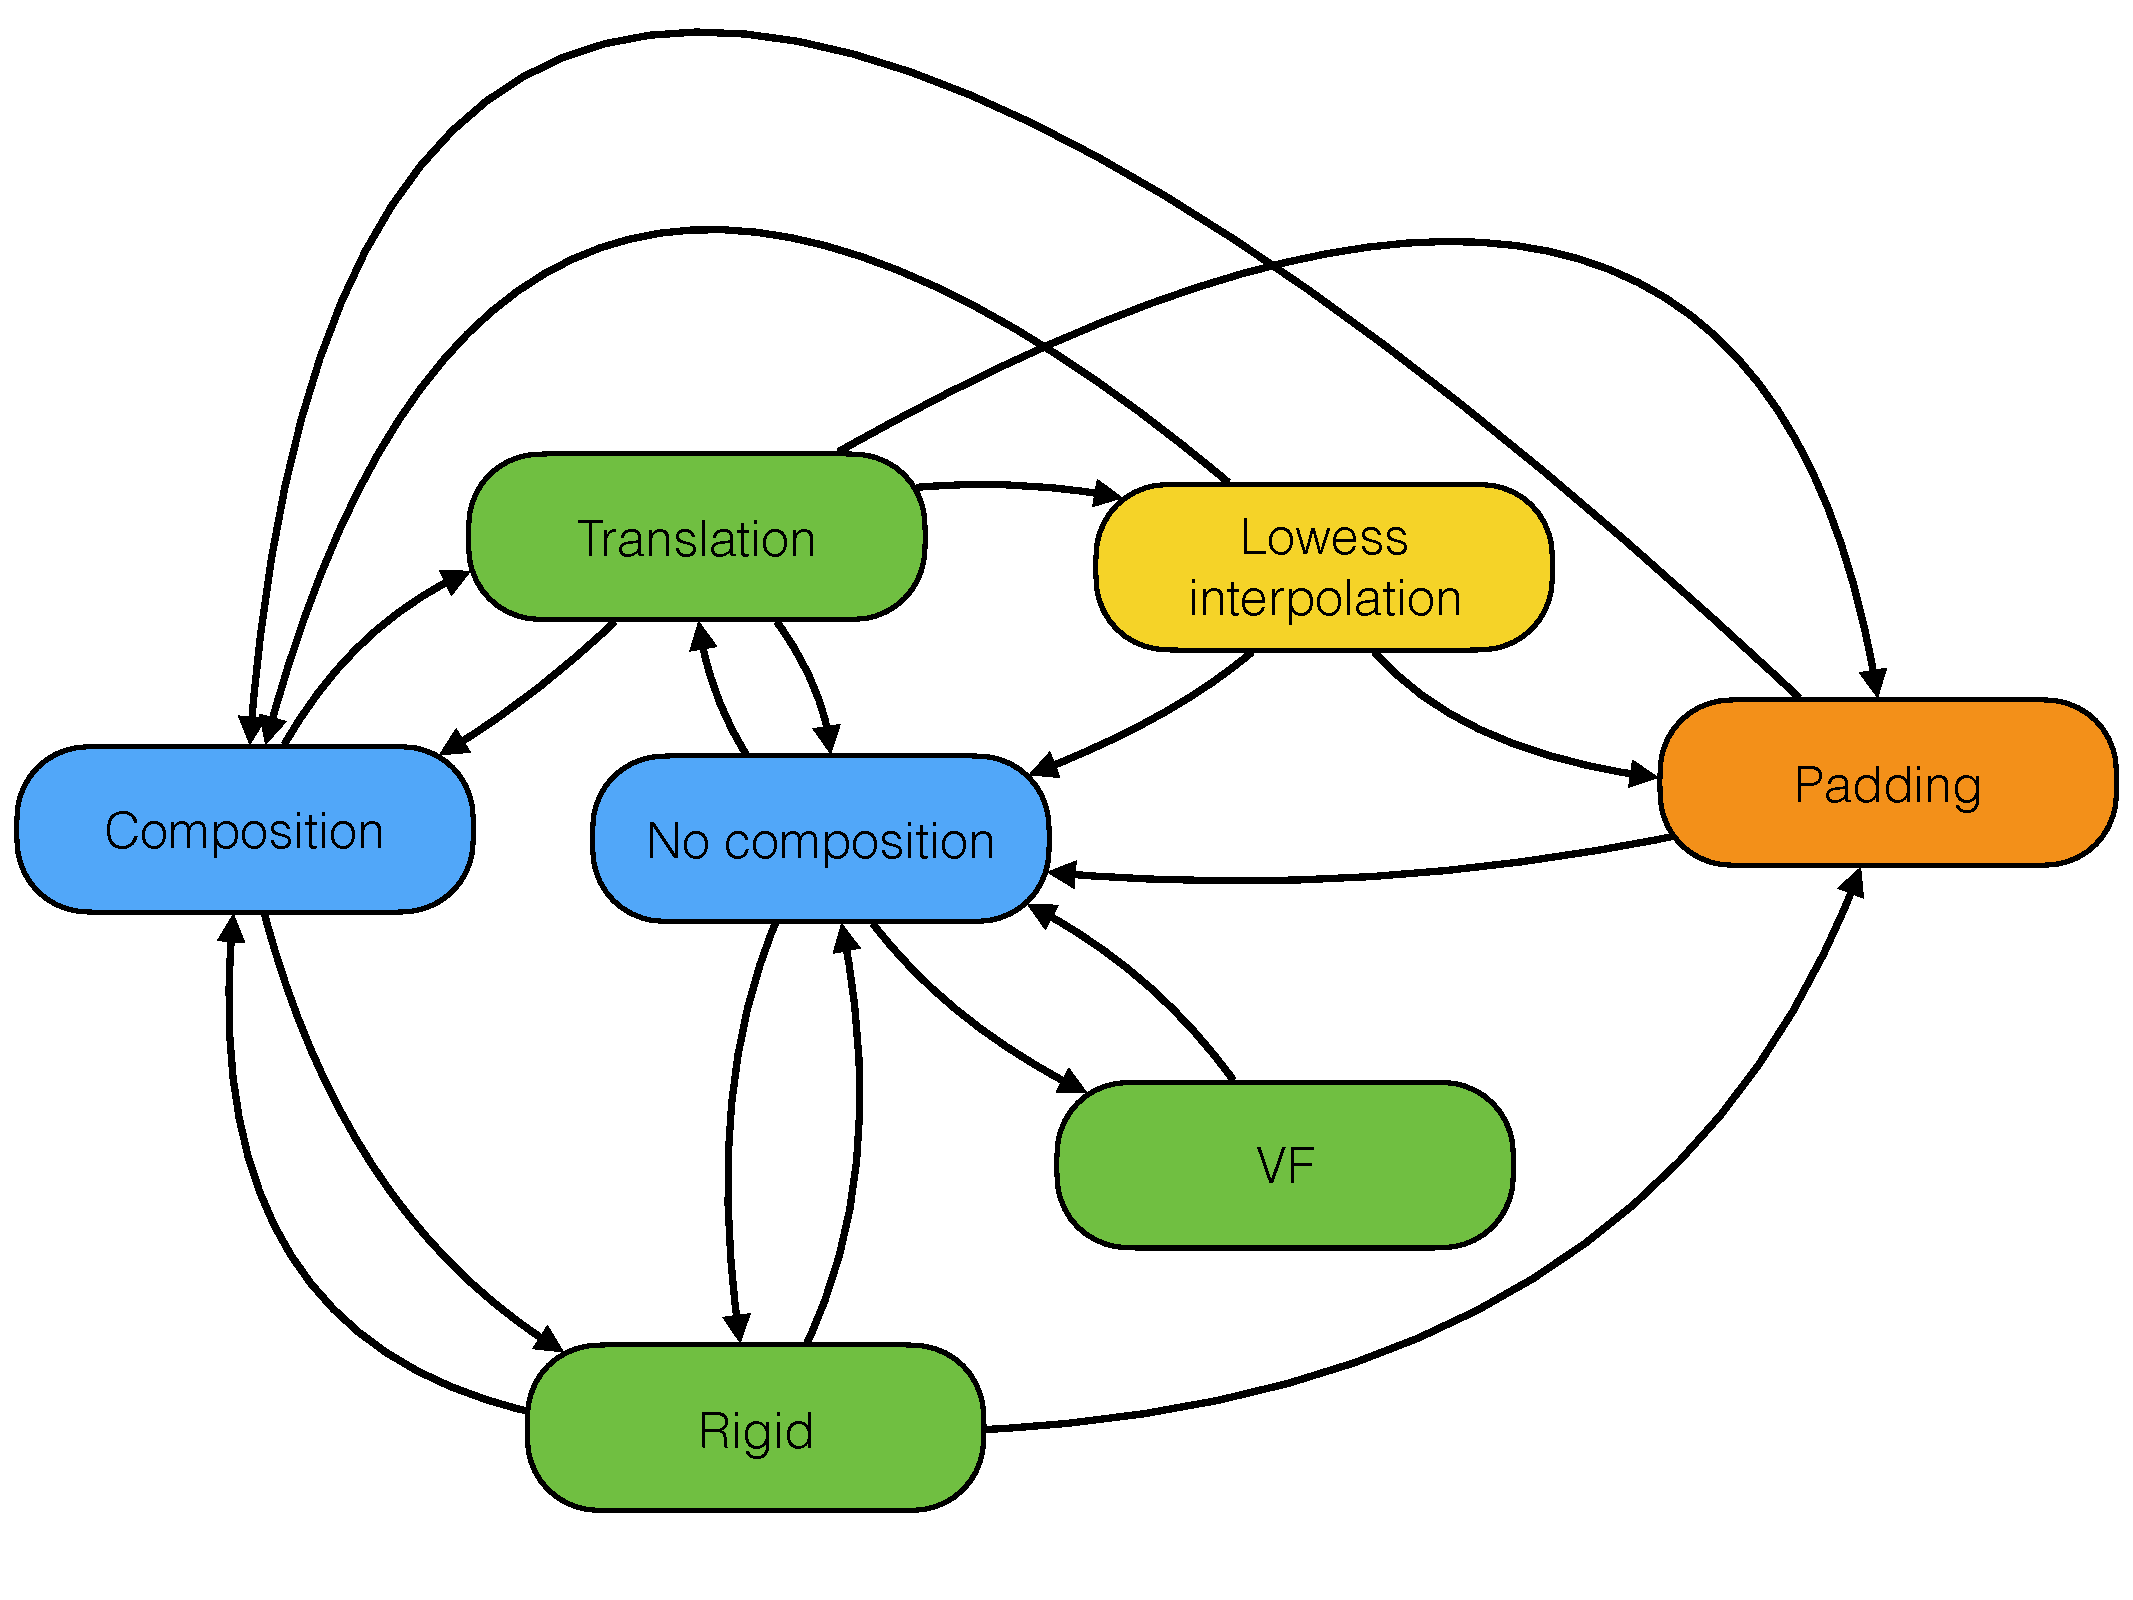
\includegraphics[width=.85\textwidth]{figures/possibilities.pdf}
  \caption{\textbf{Graph of the possible combinations} Start from one of the blue nodes, if you can go back to it, you can do it!}\label{fig:poss}
\end{figure}
\section{Configuration file examples}
\subsection{Long movies where the sample is not fixed}
Description of environment:
\begin{itemize}
\item[-] We want to compute and apply the transformations with a trilinear interpolation
\item[-] Path to images: \texttt{/path/to/time/series/T018/CH00-T0018.tif} (for time 18)
\item[-] Time points: 0 to 200, time points 23 and 145 are defections and should be discarded.
\item[-] The output transformation files will be in \texttt{/path/to/output/trsf/}
\item[-] The output registered images will be in the folder \texttt{/path/to/time/series/T018/} and the registered image will be named \texttt{CH00-T0018-rigid.klb} (for time 18)
\item[-] The output registered maximum intensity projection will be in \texttt{/path/to/output/projection/}
\item[-] The voxel size of the image in x, y, z is respectively 0.593, 0.893, 5.
\item[-] The chosen reference time point is time 100
\item[-] At most rigid transformation will be computed
\item[-] The transformations will be computed from $t_n$ to $t_{n\pm 1}$ then composed
\item[-] We want the images to be padded
\end{itemize}
Json file:
\begin{code}{0.8}
\{\\
\tab"path\_to\_data":"/path/to/time/series/T\{t:03d\}/",\\
\tab"file\_name":"CH00-T\{t:04d\}.tif",\\
\tab"trsf\_folder":"/path/to/output/trsf/",\\
\tab"output\_format":"CH00-T\{t:04d\}-rigid.klb",\\
\tab"projection\_path":"/path/to/output/projection/",\\
\tab"check\_TP":1,\\
\tab"voxel\_size":[\\
\tab\tab0.593,\\
\tab\tab0.893,\\
\tab\tab5\\
\tab],\\
\tab"first":0,\\
\tab"last":200,\\
\tab"compute\_trsf":1,\\
\tab"ref\_TP":100,\\
\tab"trsf\_type":"rigid",\\
\tab"not\_to\_do":[\\
\tab\tab23,\\
\tab\tab145\\
\tab],\\
\tab"padding":1,\\
\tab"apply\_trsf":1\\
\}
\end{code}
\subsection{Long movies where the sample is fixed}
Description of environment:
\begin{itemize}
\item[-] We want to compute and apply the transformations with cubic spline interpolation
\item[-] Path to images: \texttt{/path/to/time/series/CH00-T0018.klb} (for time 18)
\item[-] Time points: 25 to 145, no time point should be discarded.
\item[-] The output transformation files will be in \texttt{/path/to/output/trsf/}
\item[-] The output registered images will be in the folder \texttt{/path/to/output/} and the registered image will be named \texttt{T18.klb} (for time 18)
\item[-] The output registered maximum intensity projection will be in \texttt{/path/to/time/series/} and named \texttt{CH00-T-1.xyprojection.klb}
\item[-] The voxel size of the image in x, y, z is respectively 1, 1, 6.
\item[-] The chosen reference time point is time 25
\item[-] Translation will be computed
\item[-] The transformations will be computed from $t_n$ to $t_{ref}$
\item[-] We want the images to be padded
\end{itemize}
Json file:
\begin{code}{0.8}
\{\\
\tab"path\_to\_data":"/path/to/time/series/",\\
\tab"file\_name":"CH00-T\{t:04d\}.klb",\\
\tab"trsf\_folder":"/path/to/output/trsf/",\\
\tab"output\_format":"/path/to/output/T\{t:d\}.klb",\\
\tab"check\_TP":1,\\
\tab"voxel\_size":[\\
\tab\tab1,\\
\tab\tab1,\\
\tab\tab6\\
\tab],\\
\tab"first":25,\\
\tab"last":145,\\
\tab"compute\_trsf":1,\\
\tab"ref\_TP":25,\\
\tab"path\_ref":"/path/to/time/series/CH00-T\{t:04d\}.klb",\\
\tab"trsf\_type":"translation",\\
\tab"padding":1,\\
\tab"apply\_trsf":1,\\
\tab"interpolation":"cspline"\\
\}
\end{code}
\subsection{Extremely large movie where the sample slowly drifts over time}
Description of environment:
\begin{itemize}
\item[-] We want to compute and apply the transformations with a trilinear interpolation
\item[-] Path to images: \texttt{/path/to/time/series/CH00-T0018.klb} (for time 18)
\item[-] Time points: 0 to 100000, no time point should be discarded.
\item[-] The output transformation files will be in \texttt{/path/to/output/trsf/}
\item[-] The output registered images will be in the folder \texttt{/path/to/output/} and the registered image will be named as the original image name\texttt{CH00-T0018.klb} (for time 18)
\item[-] The output registered maximum intensity projection will be in \texttt{/path/to/time/series/} and named \texttt{CH00-T-1.xyprojection.klb}
\item[-] The voxel size of the image in x, y, z is respectively 1, 1, 6.
\item[-] The chosen reference time point is time 25
\item[-] We only want to compute the transformation every other 100 time point and apply a lowess smoothing with a smoothing window size of 5
\item[-] Translation will be computed
\item[-] The transformations will be computed from $t_n$ to $t_{ref}$
\item[-] We don't want the images to be padded
\end{itemize}
Json file:
\begin{code}{0.8}
\{\\
\tab"path\_to\_data":"/path/to/time/series/",\\
\tab"file\_name":"CH00-T\{t:04d\}.klb",\\
\tab"trsf\_folder":"/path/to/output/trsf/",\\
\tab"output\_format":"/path/to/output/",\\
\tab"check\_TP":1,\\
\tab"voxel\_size":[\\
\tab\tab1,\\
\tab\tab1,\\
\tab\tab6\\
\tab],\\
\tab"first":0,\\
\tab"last":100000,\\
\tab"compute\_trsf":1,\\
\tab"ref\_TP":25,\\
\tab"path\_ref":"/path/to/time/series/CH00-T\{t:04d\}.klb",\\
\tab"trsf\_type":"translation",\\
\tab"lowess\_interpolation":1,\\
\tab"window\_size":5,\\
\tab"step\_size":100,\\
\tab"padding":0,\\
\tab"apply\_trsf":1\\
\}
\end{code}
\subsection{Correcting for non linear biological movements}
Description of environment:
\begin{itemize}
\item[-] We want to compute and apply the transformations with a cubic spline interpolation
\item[-] Path to images: \texttt{/path/to/time/series/CH00-T0018.klb} (for time 18)
\item[-] Time points: 0 to 200, no time point should be discarded.
\item[-] The output transformation files will not be written (option available only for non-linear registration)
\item[-] The output registered images will be in the original folder \texttt{/path/to/time/series/} and the registered image will be named as the original with the suffix \texttt{NL}: \texttt{CH00-T0018.NL.klb} (for time 18)
\item[-] No maximum intensity projection
\item[-] The voxel size of the image in x, y, z is respectively 1, 1, 6.
\item[-] The chosen reference time point is time 25
\item[-] Non-linear transformation will be computed (preceded by a first approximation using affine registration, mandatory) with a sigma of 2.5, a registration depth of 4.
\item[-] The transformations will be computed from $t_n$ to $t_{ref}$
\item[-] We don't want the images to be padded (not possible with non-linear transformations)
\end{itemize}
Json file:
\begin{code}{0.8}
\{\\
\tab"path\_to\_data":"/path/to/time/series/",\\
\tab"file\_name":"CH00-T\{t:04d\}.klb",\\
\tab"trsf\_folder":"/path/to/output/trsf/",\\
\tab"suffix":"NL",\\
\tab"check\_TP":1,\\
\tab"voxel\_size":[\\
\tab\tab1,\\
\tab\tab1,\\
\tab\tab6\\
\tab],\\
\tab"first":0,\\
\tab"last":200,\\
\tab"compute\_trsf":1,\\
\tab"ref\_TP":25,\\
\tab"path\_ref":"/path/to/time/series/CH00-T\{t:04d\}.klb",\\
\tab"trsf\_type":"vectorfield",\\
\tab"registration\_depth":4,\\
\tab"keep\_vectorfield":0,\\
\tab"sigma":2.5,\\
\tab"padding":0,\\
\tab"apply\_trsf":1,\\
\tab"interpolation":"cspline"\\
\}
\end{code}
\subsection{Some special scenarios that could happen}
\subsubsection{Computing the transformations on one channel and applying them onto a second one.}
Description of environment:
\begin{itemize}
\item[-] We want to compute and apply the transformations on \texttt{/path/to/time/series/CH00-T0018.klb}
\item[-] and apply the transformations with a tri-linear interpolation on \texttt{/path/to/time/series/CH01-T0018.klb}
\item[-] Time points: 0 to 200, no time point should be discarded.
\item[-] The output transformation files will be in \texttt{/path/to/output/trsf/}
\item[-] The output registered images will be in the folder \texttt{/path/to/time/series/T018/} and the registered image will be named \texttt{CH00-T0018-rigid.klb} (for time 18) for \texttt{CH00} and \texttt{CH01-T0018-rigid.klb} for \texttt{CH01}
\item[-] The output registered maximum intensity projection will be in \texttt{/path/to/output/projection/}
\item[-] The voxel size of the image in x, y, z is respectively 1, 1, 5.
\item[-] The chosen reference time point is time 100
\item[-] At most rigid transformation will be computed
\item[-] The transformations will be computed from $t_n$ to $t_{n\pm 1}$ then composed
\item[-] We want the images to be padded
\end{itemize}
Json file for \texttt{CH00}:
\begin{code}{0.8}
\{\\
\tab"path\_to\_data":"/path/to/time/series/",\\
\tab"file\_name":"CH00-T\{t:04d\}.klb",\\
\tab"trsf\_folder":"/path/to/output/trsf/",\\
\tab"output\_format":"CH00-T\{t:04d\}-rigid.klb",\\
\tab"projection\_path":"/path/to/output/projection/",\\
\tab"check\_TP":1,\\
\tab"voxel\_size":[\\
\tab\tab1,\\
\tab\tab1,\\
\tab\tab5\\
\tab],\\
\tab"first":0,\\
\tab"last":200,\\
\tab"compute\_trsf":1,\\
\tab"ref\_TP":100,\\
\tab"trsf\_type":"rigid",\\
\tab"padding":1,\\
\tab"apply\_trsf":1\\
\}
\end{code}
Json file for \texttt{CH01}:
\begin{code}{0.8}
\{\\
\tab"path\_to\_data":"/path/to/time/series/",\\
\tab"file\_name":"CH01-T\{t:04d\}.klb",\\
\tab"trsf\_folder":"/path/to/output/trsf/",\\
\tab"output\_format":"CH01-T\{t:04d\}-rigid.klb",\\
\tab"projection\_path":"/path/to/output/projection/",\\
\tab"check\_TP":1,\\
\tab"voxel\_size":[\\
\tab\tab1,\\
\tab\tab1,\\
\tab\tab5\\
\tab],\\
\tab"first":0,\\
\tab"last":200,\\
\tab"compute\_trsf":0,\\
\tab"apply\_trsf":1\\
\}
\end{code}
\bibliography{biblio}
\bibliographystyle{apalike}
\end{document}
